\documentclass[12pt,a4paper]{article}

% ==================== 基础宏包 ====================
\usepackage[UTF8]{ctex}
\usepackage[margin=2.2cm]{geometry}
\usepackage{amsmath,amssymb,amsthm,mathtools}
\usepackage{array}
\usepackage{booktabs}
\usepackage{enumitem}
\usepackage{xcolor}
\usepackage{graphicx}
\usepackage{fancyhdr}
\usepackage{lastpage}
\usepackage{hyperref}
\usepackage[most]{tcolorbox}
\usepackage{titlesec}
\usepackage{tabularx}
\usepackage{listings}
\lstdefinestyle{rcode}{
  language=R,
  basicstyle=\ttfamily\footnotesize,
  keywordstyle=\color{mainblue},
  commentstyle=\color{textgray},
  stringstyle=\color{mainblue},
  breaklines=true,
  columns=fullflexible,
  keepspaces=true,
  showstringspaces=false,
  frame=single,
  rulecolor=\color{linegray},
  numbers=left,
  numberstyle=\tiny\color{textgray},
  xleftmargin=2em
}

\hypersetup{
  hidelinks
}

% ==================== 颜色定义 ====================
\definecolor{mainblue}{RGB}{34,72,112}
\definecolor{lightblue}{RGB}{241,246,252}
\definecolor{linegray}{RGB}{210,218,228}
\definecolor{textgray}{RGB}{90,98,108}

% ==================== 页面设置 ====================
\setlength{\parindent}{2em}
\setlength{\parskip}{0.35em}
\setlength{\headheight}{25pt}
\linespread{1.2}

\pagestyle{fancy}
\fancyhf{}
\lhead{\textcolor{textgray}{\small 高维数据分析课程作业}}
\rhead{\textcolor{textgray}{\small \thepage/\pageref*{LastPage}}}
\cfoot{}
\renewcommand{\headrulewidth}{0.4pt}
\renewcommand{\headrule}{%
  \hbox to\headwidth{\color{linegray}\leaders\hrule height \headrulewidth\hfill}}

% ==================== 标题样式 ====================
\titleformat{\section}
  {\Large\bfseries\color{mainblue}}
  {\thesection}
  {0.6em}
  {}

\titleformat{\subsection}
  {\large\bfseries\color{mainblue}}
  {\thesubsection}
  {0.6em}
  {}

\titlespacing*{\section}{0pt}{1.2em}{0.6em}
\titlespacing*{\subsection}{0pt}{0.8em}{0.4em}

% ==================== 自定义环境 ====================
\newtcolorbox{infobox}{
  colback=lightblue,
  colframe=mainblue,
  boxrule=0.6pt,
  arc=2mm,
  left=1.2em,
  right=1.2em,
  top=0.8em,
  bottom=0.8em
}

\newtcolorbox{answerbox}{
  colback=white,
  colframe=linegray,
  boxrule=0.5pt,
  arc=2mm,
  left=1em,
  right=1em,
  top=0.8em,
  bottom=0.8em,
  breakable
}

% ==================== 作业信息 ====================
\newcommand{\course}{高维数据分析}
\newcommand{\homeworktitle}{第1次作业}
\newcommand{\studentname}{倪伟丰}
\newcommand{\studentid}{2024110089}
\newcommand{\classname}{24 大数据 2 班}
\newcommand{\teacher}{袁洪松}
\newcommand{\duedate}{2026年10月8日}
\newcommand{\totalpoints}{150}

% ==================== 正文开始 ====================
\begin{document}

\begin{center}
  {\Huge\bfseries\color{mainblue}\homeworktitle}\\[0.6em]
  {\Large\course}\\[1.2em]
  {\color{linegray}\rule{0.9\textwidth}{0.8pt}}
\end{center}

\begin{infobox}
\begin{tabularx}{\textwidth}{>{\bfseries}p{2.2cm} X >{\bfseries}p{2.2cm} X}
姓名 & \studentname & 学号 & \studentid \\
班级 & \classname & 教师 & \teacher \\
截止时间 & \duedate & 总分 & \totalpoints 分
\end{tabularx}
\end{infobox}

% ==================================================

\section{Problem 1（15 分）}

对于样本 $(x_1,y_1),\ldots,(x_n,y_n)$，使用最小二乘法得到估计
$\hat{\beta}_0,\hat{\beta}_1$。假设拟合值为
\[
  \hat{y}_i=\hat{\beta}_0+\hat{\beta}_1x_i.
\]
试证明以下结论：
\begin{enumerate}[label=\arabic*., leftmargin=2em]
  \item $\displaystyle \frac{1}{n}\sum_{i=1}^{n}\hat{y}_i=\bar{y}$。
  \item $\displaystyle \mathrm{SS}_{\mathrm{reg}}
    =\sum_{i=1}^{n}(\hat{y}_i-\bar{y})^2$。
  \item $\displaystyle R^2=r_{XY}^2$，其中
    $\displaystyle r_{XY}^2=\frac{S_{XY}^2}{S_{XX}\cdot S_{YY}}$。
\end{enumerate}

\begin{answerbox}
\textbf{解：}

\textbf{(1)}

由 $\hat{y}_i=\hat{\beta}_0+\hat{\beta}_1x_i$，又由 $\sum_{i=1}^{n}\hat{e}_i=0$ 可得 $\hat{\beta}_0=\bar{y}-\hat{\beta}_1\bar{x}$，故：

$$
\frac{1}{n}\sum_{i=1}^{n}\hat{y}_i=\frac{1}{n}\sum_{i=1}^{n}\left(\hat{\beta}_0+\hat{\beta}_1x_i\right)=\frac{1}{n}\sum_{i=1}^{n}\left(\bar{y}-\hat{\beta}_1\bar{x}+\hat{\beta}_1x_i\right)=\bar{y}-\hat{\beta}_1\bar{x}+\hat{\beta}_1\cdot\frac{1}{n}\sum_{i=1}^{n}x_i=\bar{y}
$$

\textbf{(2)}

由定义，$\mathrm{SS}_{\mathrm{reg}}=S_{YY}-\mathrm{RSS}$，其中 $S_{YY}=\sum_{i=1}^{n}(y_i-\bar{y})^2$，$\mathrm{RSS}=\sum_{i=1}^{n}(y_i-\hat{y}_i)^2$。

又：

$$
\hat{y}_i-\bar{y}=\hat{\beta}_0+\hat{\beta}_1x_i-\bar{y}=\bar{y}-\hat{\beta}_1\bar{x}+\hat{\beta}_1x_i-\bar{y}=\hat{\beta}_1(x_i-\bar{x})
$$

于是：

$$
\begin{aligned}
\mathrm{SS}_{\mathrm{reg}}=&\sum_{i=1}^{n}(y_i-\bar{y})^2-\sum_{i=1}^{n}(y_i-\hat{y_i})^2 \\
=& \sum_{i=1}^{n}(y_i-\hat{y_i}+\hat{y_i}-\bar{y})^2-\sum_{i=1}^{n}(y_i-\hat{y_i})^2 \\
=& \sum_{i=1}^{n}(y_i-\hat{y_i})^2 + 2 \sum_{i=1}^{n}(y_i-\hat{y_i})(\hat{y_i}-\bar{y}) + \sum_{i=1}^{n}(\hat{y_i}-\bar{y})^2-\sum_{i=1}^{n}(y_i-\hat{y_i})^2 \\
=& 2 \sum_{i=1}^{n}(y_i-\hat{y_i})(\hat{y_i}-\bar{y}) + \sum_{i=1}^{n}(\hat{y_i}-\bar{y})^2
\end{aligned}
$$

其中：

$$
\begin{aligned}
\sum_{i=1}^{n}(y_i-\hat{y_i})(\hat{y_i}-\bar{y}) =& \sum_{i=1}^{n}\hat{e_i}\hat{\beta}_1(x_i-\bar{x}) \\
=&\hat{\beta_1}\sum_{i=1}^{n}\hat{e}_ix_i - \hat{\beta_1}\bar{x}\sum_{i=1}^{n}\hat{e_i}
\end{aligned}
$$

最小二乘估计 $(\hat{\beta}_0,\hat{\beta}_1)$ 使残差平方和

$$
f(\beta_0,\beta_1)=\sum_{i=1}^n(y_i-\beta_0-\beta_1x_i)^2
$$

达到最小，其中 $\hat{e}_i=y_i-\hat{\beta}_0-\hat{\beta}_1x_i$。由于模型含有截距项，对目标函数关于 $\beta_0$ 求偏导，并在最小二乘估计处令其为零，得到：

$$
\left.\frac{\partial f}{\partial\beta_0}\right|_{(\hat\beta_0,\hat\beta_1)}
=-2\sum_{i=1}^n(y_i-\hat\beta_0-\hat\beta_1x_i)
=-2\sum_{i=1}^n\hat{e}_i=0
$$

因此 $\sum_{i=1}^n\hat{e}_i=0$。同理，对目标函数关于 $\beta_1$ 求偏导，并在最小二乘估计处令其为零：

$$
\left.\frac{\partial f}{\partial\beta_1}\right|_{(\hat\beta_0,\hat\beta_1)} =-2\sum_{i=1}^n (y_i-\hat\beta_0-\hat\beta_1x_i)x_i =-2\sum_{i=1}^n \hat{e}_ix_i = 0
$$

于是：

$$
\sum_{i=1}^n \hat{e}_ix_i = 0
$$

所以：

$$
\sum_{i=1}^{n}(y_i-\hat{y_i})(\hat{y_i}-\bar{y})
=\hat{\beta_1}\sum_{i=1}^{n}\hat{e}_ix_i - \hat{\beta_1}\bar{x}\sum_{i=1}^{n}\hat{e_i}
=0-0=0
$$

回代：

$$
\mathrm{SS}_{\mathrm{reg}}= 2 \sum_{i=1}^{n}(y_i-\hat{y_i})(\hat{y_i}-\bar{y}) + \sum_{i=1}^{n}(\hat{y_i}-\bar{y})^2=\sum_{i=1}^{n}(\hat{y_i}-\bar{y})^2
$$

\textbf{(3)}

$$
\sum_{i=1}^{n}(\hat{y}_i-\bar{y})^2=\sum_{i=1}^{n}\hat{\beta}_1^2(x_i-\bar{x})^2=\hat{\beta}_1^2 S_{XX}=\frac{S_{XY}^2}{S_{XX}^2}\cdot S_{XX}=\frac{S_{XY}^2}{S_{XX}}
$$

由第 (2) 小问结论：

$$
\mathrm{SS}_{\mathrm{reg}} = \sum_{i=1}^{n}(\hat{y}_i-\bar{y})^2
$$


所以：

$$
S_{YY}-\mathrm{RSS}=\frac{S_{XY}^2}{S_{XX}}
$$

左右除以 $S_{YY}$ 得到：

$$
1-\frac{\mathrm{RSS}}{S_{YY}}=\frac{S_{XY}^2}{S_{XX}\cdot S_{YY}}
$$

由 $R^2$ 的定义 $R^2=1-\dfrac{\mathrm{RSS}}{S_{YY}}$，也就是说：

$$
R^2=r^2_{XY}
$$

\end{answerbox}

% ==================================================

\section{Problem 2（10 分）}

假设有一个没有截距的线性模型
\[
  y_i=\beta^*x_i+e_i,\qquad i=1,\ldots,n,
\]
其中 $e_1,\ldots,e_n$ 为 i.i.d.\ $N(0,\sigma_*^2)$ 的随机变量。
考虑 $\beta^*$ 的最小二乘估计量 $\hat{\beta}$（最小二乘法中也不考虑截距），
以及另一个估计量
\[
  \widetilde{\beta}=\frac{\bar{y}}{\bar{x}}.
\]

\subsection{}

证明 $\hat{\beta}$ 与 $\widetilde{\beta}$ 均为 $\beta^*$ 的无偏估计。

\begin{answerbox}
\textbf{解：}

由最小二乘法，$\hat{\beta}$ 最小化目标函数：

$$
Q(\beta)=\sum_{i=1}^{n}(y_i-\beta x_i)^2
$$

令 $\dfrac{\partial Q}{\partial\beta}=-2\sum_{i=1}^{n}(y_i-\beta x_i)x_i=0$（由 $x_i$ 不全为 $0$，$S_X>0$），解得：

$$
\hat{\beta}=\frac{\sum_{i=1}^{n}x_iy_i}{\sum_{i=1}^{n}x_i^2}
$$

由于 $S_X>0$，且假设 $\bar{x}\neq 0$，令：

$$
S_X=\sum_{i=1}^{n}x_i^2, \quad c_i=\frac{x_i}{S_X}, \quad d_i = \frac{1}{n\bar{x}}
$$

于是：

$$
\sum_{i=1}^{n}c_ix_i=\frac{1}{S_X}\sum_{i=1}^{n}x_i^2=1, \quad \sum_{i=1}^{n}d_ix_i=\frac{1}{n\bar{x}}\sum_{i=1}^{n}x_i=1
$$

$$
\sum_{i=1}^{n}c_i^2=\sum_{i=1}^{n}\frac{x_i^2}{S_X^2}=\frac{1}{S_X}, \quad \sum_{i=1}^{n}d_i^2=n\left(\frac{1}{n\bar{x}}\right)^2=\frac{n}{\left(\sum_{i=1}^{n}x_i\right)^2}
$$

由 $E[e_i]=0$ 得 $E[y_i]=\beta^*x_i$，分别计算期望：

$$
E\hat{\beta}=E\left[\sum_{i=1}^{n}c_iy_i\right]=\sum_{i=1}^{n}c_iE[y_i]=\beta^*\sum_{i=1}^{n}c_ix_i=\beta^*
$$

$$
E\widetilde{\beta}=E\left[\sum_{i=1}^{n}d_iy_i\right]=\sum_{i=1}^{n}d_iE[y_i]=\beta^*\sum_{i=1}^{n}d_ix_i=\beta^*
$$

所以，$\hat{\beta}$ 与 $\widetilde{\beta}$ 均为 $\beta^*$ 的无偏估计量。

\end{answerbox}

\subsection{}

试比较 $\hat{\beta}$ 与 $\widetilde{\beta}$ 哪个方差更小。

\begin{answerbox}
\textbf{解：}

由 $e_1,\ldots,e_n$ i.i.d.\ 可知 $y_1,\ldots,y_n$ 相互独立，且 $\operatorname{Var}(y_i)=\sigma_*^2$。于是：

$$
\operatorname{Var}\left(\hat{\beta}\right)=\operatorname{Var}\left(\sum_{i=1}^{n}c_iy_i\right)=\sum_{i=1}^{n}c_i^2\operatorname{Var}\left(y_i\right)=\sigma_*^2\sum_{i=1}^{n}\frac{x_i^2}{S_X^2}=\frac{\sigma_*^2}{S_X}
$$

$$
\operatorname{Var}\left(\widetilde{\beta}\right)=\operatorname{Var}\left(\sum_{i=1}^{n}d_iy_i\right)=\sum_{i=1}^{n}d_i^2\operatorname{Var}\left(y_i\right)=\sigma_*^2\cdot n\left(\frac{1}{n\bar{x}}\right)^2=\frac{n\,\sigma_*^2}{\left(\sum_{i=1}^{n}x_i\right)^2}
$$

由 Cauchy--Schwarz 不等式：

$$
\left(\sum_{i=1}^{n}x_i\right)^2\le n\sum_{i=1}^{n}x_i^2=nS_X
$$

所以：

$$
\operatorname{Var}\left(\widetilde{\beta}\right)=\frac{n\,\sigma_*^2}{\left(\sum_{i=1}^{n}x_i\right)^2}\ge\frac{\sigma_*^2}{S_X}=\operatorname{Var}\left(\hat{\beta}\right)
$$

即 $\operatorname{Var}\left(\hat{\beta}\right)\le\operatorname{Var}\left(\widetilde{\beta}\right)$，$\hat{\beta}$ 的方差更小（或相等）；等号当且仅当所有 $x_i$ 都相等时成立。

\end{answerbox}

% ==================================================

\section{Problem 3（30 分）}

考虑一个简单线性回归模型。已知
\[
  n=25,\qquad \bar{x}=2.8,\qquad \bar{y}=-3.4,\qquad
  S_{XX}=586,\qquad S_{XY}=-1725,\qquad S_{YY}=5099,
\]
且 $\mathrm{RSS}=21.06$。

\textit{（此题不是代码题，写清计算过程及结果即可。）}

\subsection{}

计算 $\hat{\beta}_0,\hat{\beta}_1,\hat{\sigma}^2$。

\begin{answerbox}
\textbf{解：}

由最小二乘估计：

$$
\hat{\beta}_1=\frac{S_{XY}}{S_{XX}}=\frac{-1725}{586}\approx-2.9437
$$

$$
\hat{\beta}_0=\bar{y}-\hat{\beta}_1\bar{x}=-3.4-(-2.9437)\times 2.8\approx 4.8423
$$

回归自由度为 $n-2=23$：

$$
\hat{\sigma}^2=\frac{\mathrm{RSS}}{n-2}=\frac{21.06}{23}\approx 0.9157,\qquad \hat{\sigma}\approx 0.9569
$$

\end{answerbox}

\subsection{}

计算 $\operatorname{se}(\hat{\beta}_0)$ 和
    $\operatorname{se}(\hat{\beta}_1)$。

\begin{answerbox}
\textbf{解：}

$$
\operatorname{se}(\hat{\beta}_1)=\frac{\hat{\sigma}}{\sqrt{S_{XX}}}=\frac{0.9569}{\sqrt{586}}\approx 0.0395
$$

对于 $\hat{\beta}_0$，由 $\hat{\beta}_0=\bar{y}-\hat{\beta}_1\bar{x}$，且由于
$\operatorname{Cov}(\bar{y},\hat{\beta}_1)=\dfrac{\sigma_*^2}{nS_{XX}}\sum_{i=1}^{n}(x_i-\bar{x})=0$，故

$$
\operatorname{Var}(\hat{\beta}_0)=\operatorname{Var}(\bar{y})+\bar{x}^2\operatorname{Var}(\hat{\beta}_1)=\sigma_*^2\left(\frac{1}{n}+\frac{\bar{x}^2}{S_{XX}}\right)
$$

将 $\sigma_*$ 换成 $\hat{\sigma}$：

$$
\operatorname{se}(\hat{\beta}_0)=\hat{\sigma}\sqrt{\frac{1}{n}+\frac{\bar{x}^2}{S_{XX}}}=0.9569\times\sqrt{0.04+\frac{2.8^2}{586}}=0.9569\times\sqrt{0.05338}\approx 0.2211
$$

\end{answerbox}

\subsection{}

对于一个新的样本，我们观测到自变量值为 $x_{\mathrm{new}}=5$，
    用
    \[
      \hat{y}_{\mathrm{new}}
      =\hat{\beta}_0+\hat{\beta}_1x_{\mathrm{new}}
    \]
    作为因变量的预测值。试计算其标准误
    $\operatorname{se}(\hat{y}_{\mathrm{new}})$。

    提示：可先按照公式
    \[
      \operatorname{Var}(\hat{\beta}_0+\hat{\beta}_1x_{\mathrm{new}})
      =\operatorname{Var}(\hat{\beta}_0)
      +x_{\mathrm{new}}^2\operatorname{Var}(\hat{\beta}_1)
      +2x_{\mathrm{new}}\operatorname{Cov}(\hat{\beta}_0,\hat{\beta}_1)
    \]
    求其方差以及标准差，再将标准差中的 $\sigma_*$ 换成 $\hat{\sigma}$
    即得到标准误。

\begin{answerbox}
\textbf{解：}
先求预测值：

$$
\hat{y}_{\mathrm{new}}=\hat{\beta}_0+\hat{\beta}_1x_{\mathrm{new}}=4.8423-2.9437\times 5\approx-9.8761
$$

再求方差：

$$
\operatorname{Var}(\hat{y}_{\mathrm{new}})=\operatorname{Var}(\hat{\beta}_0)+x_{\mathrm{new}}^2\operatorname{Var}(\hat{\beta}_1)+2x_{\mathrm{new}}\operatorname{Cov}(\hat{\beta}_0,\hat{\beta}_1)
$$

其中由 $\hat{\beta}_0=\bar{y}-\hat{\beta}_1\bar{x}$ 及 $\operatorname{Cov}(\bar{y},\hat{\beta}_1)=0$：

$$
\operatorname{Cov}(\hat{\beta}_0,\hat{\beta}_1)=\operatorname{Cov}(\bar{y},\hat{\beta}_1)-\bar{x}\operatorname{Var}(\hat{\beta}_1)=-\frac{\bar{x}}{S_{XX}}\sigma_*^2
$$

代入并化简：

$$
\operatorname{Var}(\hat{y}_{\mathrm{new}})=\sigma_*^2\left(\frac{1}{n}+\frac{\bar{x}^2}{S_{XX}}\right)+\frac{x_{\mathrm{new}}^2}{S_{XX}}\sigma_*^2-\frac{2x_{\mathrm{new}}\bar{x}}{S_{XX}}\sigma_*^2=\sigma_*^2\left(\frac{1}{n}+\frac{(x_{\mathrm{new}}-\bar{x})^2}{S_{XX}}\right)
$$

代入数值：

$$
\operatorname{Var}(\hat{y}_{\mathrm{new}})=0.9157\times\left(0.04+\frac{(5-2.8)^2}{586}\right)=0.9157\times\left(0.04+0.00826\right)\approx 0.04419
$$

将 $\sigma_*$ 换成 $\hat{\sigma}$ 后开方：

$$
\operatorname{se}(\hat{y}_{\mathrm{new}})=\sqrt{0.04419}\approx 0.2102
$$
\end{answerbox}

% ==================================================

\section{Problem 4（15 分）}

假设一个多元线性回归模型中
\[
  n=153,\qquad p=2,\qquad S_{YY}=1067.3,\qquad \mathrm{RSS}=600.
\]
另外知道
\[
  (X^\mathsf{T}X)^{-1}
  =
  \begin{pmatrix}
    4.42654 & -1.46 & 0.36 \\
    -1.46   & 0.50  & -0.20 \\
    0.36    & -0.20 & 0.40
  \end{pmatrix},
  \qquad
  X^\mathsf{T}Y
  =
  \begin{pmatrix}
    10679 \\
    34196 \\
    7512
  \end{pmatrix}.
\]


\textit{（此题不是代码题，写清计算过程及结果即可。）}

\subsection{}

求出估计量 $\hat{\beta}_1$，以及 $\beta_1^*$ 置信度为 $95\%$
    的置信区间。

\begin{answerbox}
\textbf{解：}

$$
\hat{\beta}=(X^\mathsf{T}X)^{-1}X^\mathsf{T}Y=\begin{pmatrix}4.42654 & -1.46 & 0.36\\ -1.46 & 0.50 & -0.20\\ 0.36 & -0.20 & 0.40\end{pmatrix}\begin{pmatrix}10679\\34196\\7512\end{pmatrix}=\begin{pmatrix}49.18\\4.26\\10.04\end{pmatrix}
$$

所以 $\hat{\beta}_1=4.26$。参数个数为 $p+1=3$，自由度为 $n-(p+1)=150$，故

$$
\hat{\sigma}^2=\frac{\mathrm{RSS}}{n-p-1}=\frac{600}{153-3}=4,\qquad \hat{\sigma}=2
$$

\textbf{枢轴量：}

$$
T=\frac{\hat{\beta}_1-\beta_1^*}{\hat{\sigma}\sqrt{\left[(X^\mathsf{T}X)^{-1}\right]_{22}}}=\frac{\hat{\beta}_1-\beta_1^*}{2\sqrt{0.50}}
$$

在模型假设下，$T\sim t(n-p-1)=t(150)$。

$P\left(T>t_\alpha(n)\right)=\alpha$。由 $P\left(|T|\le t_{0.025}(150)\right)=0.95$，得 $\beta_1^*$ 的置信度为 $95\%$ 的置信区间

$$
\left[\hat{\beta}_1-t_{0.025}(150)\cdot 2\sqrt{0.50},\;\;\hat{\beta}_1+t_{0.025}(150)\cdot 2\sqrt{0.50}\right]
$$

带入数值：

$$
\left[4.26-t_{0.025}(150)\cdot\sqrt{2},\;\;4.26+t_{0.025}(150)\cdot\sqrt{2}\right]
$$

\end{answerbox}

\subsection{}

在 $1\%$ 的显著水平下检验 $\beta_2^*$ 是否显著非零。

\begin{answerbox}
\textbf{解：}

写出假设检验：

$$
H_0:\;\beta_2^*=0\qquad\text{vs.}\qquad H_1:\;\beta_2^*\neq 0,\qquad \alpha=0.01
$$

于是可以写出检验统计量：

$$
T=\frac{\hat{\beta}_2}{\hat{\sigma}\sqrt{\left[(X^\mathsf{T}X)^{-1}\right]_{33}}}=\frac{\hat{\beta}_2}{2\sqrt{0.40}}
$$

在 $H_0$ 成立时 $T\sim t(n-p-1)=t(150)$。

所以拒绝域是：

$$
|T|>t_{0.005}(150)
$$

带入数值，由 $2\sqrt{0.40}\approx 1.2649$，

$$
T=\frac{10.04}{1.2649}\approx 7.94
$$

由于 $|T|\approx 7.94>t_{0.005}(150)$，落在拒绝域内，故拒绝 $H_0$，即认为 $\beta_2^*$ 显著非零。
\end{answerbox}

\subsection{}

计算回归的 $R^2$。

\begin{answerbox}
\textbf{解：}

$$
R^2=1-\frac{\mathrm{RSS}}{S_{YY}}=1-\frac{600}{1067.3}\approx 0.4378
$$
\end{answerbox}

% ==================================================

\section{Problem 5（10 分）}

假设有两个自变量、一个因变量，观测到的样本为
\[
  (x_{11},x_{12},y_1),\ldots,(x_{n1},x_{n2},y_n).
\]
首先做最小二乘法，即求
\[
  \min_{\beta_0,\beta_1,\beta_2}
  \sum_{i=1}^{n}
  (y_i-\beta_0-\beta_1x_{i1}-\beta_2x_{i2})^2.
\]
假设回归的 RSS 记为 $\mathrm{rss}$，$R^2$ 记为 $r^2$。

其次，只将第一个自变量包含进来做最小二乘法，即求
\[
  \min_{\beta_0,\beta_1}
  \sum_{i=1}^{n}(y_i-\beta_0-\beta_1x_{i1})^2.
\]
假设如此做得到的 RSS 为 $\mathrm{rss}_0$，$R^2$ 为 $r_0^2$。

\subsection{}

比较 $\mathrm{rss}$ 与 $\mathrm{rss}_0$ 的大小。

\begin{answerbox}
\textbf{解：}

首先记残差平方和为

$$
\mathrm{rss}(\beta_0, \beta_1, \beta_2) = \sum_{i=1}^{n}
  (y_i-\beta_0-\beta_1x_{i1}-\beta_2x_{i2})^2.
$$

把两个最小二乘问题写成对参数空间求最小值。

完整模型的参数空间为

$$
\Theta =\left\{(\beta_0, \beta_1, \beta_2): \beta_0, \beta_1, \beta_2 \in \mathbb{R} \right\} = \mathbb{R}^3,
$$

简化模型对应的参数集合为

$$
\Theta_0 =\left\{(\beta_0, \beta_1, 0): \beta_0, \beta_1 \in \mathbb{R} \right\} \subset \Theta.
$$

也就是说，简化模型的最优解是完整模型的可行解。

简化模型等价于：

$$
\begin{aligned}
\min_{\beta_0, \beta_1, \beta_2}\quad & \sum_{i=1}^{n}
  (y_i-\beta_0-\beta_1x_{i1}-\beta_2x_{i2})^2 \\
\text{s.t.}\quad & \beta_2 = 0,\qquad \beta_0, \beta_1 \in \mathbb{R}
\end{aligned}
$$

对于简化模型的最优解 $\boldsymbol{\beta}^{\dagger} = (\beta_0^{\dagger}, \beta_1^{\dagger}, 0)^{\mathsf{T}}$，它自然也是完整模型的可行解。

而完整模型的最优解为 $\hat{\boldsymbol{\beta}} = (\hat{\beta}_0, \hat{\beta}_1, \hat{\beta}_2)^{\mathsf{T}}$，一定有：

$$
\mathrm{rss} = \mathrm{rss}(\hat{\boldsymbol{\beta}}) \leq \mathrm{rss}(\boldsymbol{\beta}^{\dagger}) = \mathrm{rss}_0
$$

所以：

$$
\mathrm{rss} \leq \mathrm{rss}_0
$$

当且仅当 $\hat{\beta}_2=0$ 时，等号成立；也就是说，当且仅当 $X_{(2)}$ 可由截距项 $1$ 与 $X_{1}$ 线性表出时，等号成立。

\end{answerbox}

\subsection{}

比较 $r^2$ 与 $r_0^2$ 的大小。

\begin{answerbox}
\textbf{解：}

$$
r^2=1-\frac{\mathrm{rss}}{S_{YY}}, \quad r_0^2=1-\frac{\mathrm{rss}_0}{S_{YY}}
$$

其中 $S_{YY}=\sum_{i=1}^{n}(y_i-\bar{y})^2$ 只与观测数据有关，与模型无关，且 $S_{YY}>0$。

由于第 1 问已证 $\mathrm{rss}_0 \geq \mathrm{rss}$，所以

$$
r^2 = 1-\frac{\mathrm{rss}}{S_{YY}} \geq 1-\frac{\mathrm{rss}_0}{S_{YY}} = r_0^2
$$

当且仅当 $\hat{\beta}_2=0$ 时，等号成立；也就是说，当且仅当 $X_{(2)}$ 可由 $1$ 与 $X_{1}$ 线性表出时，等号成立。

\end{answerbox}

% ==================================================

\section{Problem 6（20 分）}

考虑 $n$ 个样本、$p$ 个变量的多元线性回归问题，样本为
$X\in\mathbb{R}^{n\times(p+1)}$、$Y\in\mathbb{R}^n$。
对于一个 $(p+1)$ 维常数向量 $c\in\mathbb{R}^{p+1}$：

\subsection{}

请找出 $c^\mathsf{T}\beta$ 的极大似然估计，并证明其无偏。

\begin{answerbox}
\textbf{解：}

先求 $\beta$ 的 MLE。假设 $X$ 列满秩（从而 $X^{\mathsf T}X$ 可逆），且 $X$ 为固定的设计矩阵。模型为
$$
Y=X\beta+e,\qquad e\sim N(0,\sigma^2 I_n),
$$
于是
$$
Y\sim N(X\beta,\ \sigma^2 I_n).
$$

有似然函数：

$$
L(\beta,\sigma^2)=\prod_{i=1}^{n}\frac{1}{\sqrt{2\pi\sigma^2}}
\exp\left(-\frac{(y_i-x_i^{\mathsf{T}}\beta)^2}{2\sigma^2}\right)
=(2\pi\sigma^2)^{-n/2}\exp\left(-\frac{1}{2\sigma^2}\|Y-X\beta\|^2\right).
$$

对数似然函数为：

$$
\ell(\beta,\sigma^2)
=-\frac{n}{2}\log(2\pi\sigma^2)-\frac{1}{2\sigma^2}\|Y-X\beta\|^2 .
$$

对固定的 $\sigma^2$，$\ell$ 关于 $\beta$ 最大化等价于最小化 $\|Y-X\beta\|^2$（关于 $\beta$ 的凸二次函数）。对 $\ell$ 关于 $\beta$ 求梯度并令其为零：
$$
\frac{\partial \ell}{\partial\beta}
=\frac{1}{\sigma^2}X^{\mathsf{T}}(Y-X\beta)=0
\quad\Longrightarrow\quad
X^{\mathsf{T}}X\beta=X^{\mathsf{T}}Y .
$$
解得
$$
\hat{\beta}=(X^{\mathsf{T}}X)^{-1}X^{\mathsf{T}}Y .
$$

由 MLE 的不变性，$c^{\mathsf T}\beta$ 的 MLE 为 $c^{\mathsf T}\hat{\beta}$。

接下来证明无偏性：

$$
\begin{aligned}
E\left[c^{\mathsf T}\hat{\beta}\right]
=&E\left[c^{\mathsf T}(X^{\mathsf T}X)^{-1}X^{\mathsf T}Y\right]=E\left[c^{\mathsf T}(X^{\mathsf T}X)^{-1}X^{\mathsf T}(X\beta+e)\right]\\
=&E\left[c^{\mathsf T}(X^{\mathsf T}X)^{-1}X^{\mathsf T}X\beta+c^{\mathsf T}(X^{\mathsf T}X)^{-1}X^{\mathsf T}e\right]\\
=&c^{\mathsf T}\beta+c^{\mathsf T}(X^{\mathsf T}X)^{-1}X^{\mathsf T}E\left[e\right]=c^{\mathsf T}\beta\quad\left(E\left[e\right]=0\right)
\end{aligned}
$$

所以，$c^{\mathsf T}\hat{\beta}$ 是 $c^{\mathsf T}\beta$ 的无偏估计量。
\end{answerbox}

\subsection{}

请计算1中得到的估计量的方差

\begin{answerbox}
\textbf{解：}

由第 1 小问，$c^{\mathsf T}\beta$ 的极大似然估计（也是最小二乘估计）为
$$
c^{\mathsf T}\hat{\beta}
=c^{\mathsf T}(X^{\mathsf T}X)^{-1}X^{\mathsf T}Y.
$$

将 $Y=X\beta+e$ 代入，得
$$
\hat{\beta}
=(X^{\mathsf T}X)^{-1}X^{\mathsf T}(X\beta+e)
=\beta+(X^{\mathsf T}X)^{-1}X^{\mathsf T}e,
$$
于是
$$
c^{\mathsf T}\hat{\beta}=c^{\mathsf T}\beta+c^{\mathsf T}(X^{\mathsf T}X)^{-1}X^{\mathsf T}e.
$$
其中 $c^{\mathsf T}\beta$ 为常数，故（$X$ 固定，记 $A=(X^{\mathsf T}X)^{-1}X^{\mathsf T}$，利用 $\operatorname{Var}(Ae)=A\operatorname{Var}(e)A^{\mathsf T}$）
$$
\begin{aligned}
\operatorname{Var}\left(c^{\mathsf T}\hat{\beta}\right)
=&\operatorname{Var}\left(c^{\mathsf T}Ae\right)
=c^{\mathsf T}A\operatorname{Var}\left(e\right)A^{\mathsf T}c\\
=&c^{\mathsf T}(X^{\mathsf T}X)^{-1}X^{\mathsf T}\operatorname{Var}\left(e\right)X(X^{\mathsf T}X)^{-1}c\\
\end{aligned}
$$
% 其中用到 $A^{\mathsf T}=X(X^{\mathsf T}X)^{-1}$（由 $(X^{\mathsf T}X)^{-1}$ 的对称性）。

又 $e\sim N(0, \sigma^2 I_n)$，所以 $\operatorname{Var}\left(e\right)=\sigma^2 I_n$，代入得

$$
\operatorname{Var}\left(c^{\mathsf T}\hat{\beta}\right)
=\sigma^2\,c^{\mathsf T}(X^{\mathsf T}X)^{-1}X^{\mathsf T}X(X^{\mathsf T}X)^{-1}c
=\sigma^2\,c^{\mathsf T}(X^{\mathsf T}X)^{-1}c.
$$
\end{answerbox}

% ==================================================

\section{Problem 7（10 分）}

\textbf{（过拟合，overfitting）}
考虑一个线性模型
\[
  Y=X\beta^*+e.
\]
由于不知道以上的真实模型，我们在做线性回归时可能会加入一些无关变量。
假设我们加入了另外的 $q$ 个变量，它们的样本值为
\[
  X'
  =
  \begin{bmatrix}
    x_{1(p+1)} & \cdots & x_{1(p+q)} \\
    \vdots     & \ddots & \vdots \\
    x_{n(p+1)} & \cdots & x_{n(p+q)}
  \end{bmatrix}.
\]
我们令
\[
  Z=[\,X\;\;X'\,],
\]
即把所有 $p+q+1$ 个变量都放进来，形成一个
$n\times(p+q+1)$ 的矩阵。同时在 $\beta^*$ 后面加入 $q$ 个 $0$，得到
\[
  b^*=(\beta_0^*,\beta_1^*,\ldots,\beta_p^*,0,\ldots,0)^\mathsf{T}.
\]
那么原模型可以等价地表示为
\[
  Y=Zb^*+e.
\]

\subsection{}

按照我们对变量的选择，最小二乘的目标为最小化
    \[
      \lVert Y-Zb\rVert^2.
    \]
试计算由此得到的一个 $b^*$ 的估计量 $\widetilde{b}$。

\begin{answerbox}
\textbf{解：}
使用最小二乘法估计$b$：

$$
\min_{b} \lVert Y-Zb\rVert^2
$$

对目标函数关于 $b$ 求梯度：

$$
\nabla_b\,\lVert Y-Zb\rVert^2=2Z^{\mathsf T}(Zb-Y)
$$

令梯度等于零：

$$
2Z^{\mathsf T}(Zb-Y)=2(Z^{\mathsf T}Zb-Z^{\mathsf T}Y)=0
\quad\Longrightarrow\quad
Z^{\mathsf T}Zb=Z^{\mathsf T}Y
$$

假设 $Z$ 列满秩（从而 $Z^{\mathsf T}Z$ 可逆），解得
$$
\widetilde{b}=(Z^{\mathsf T}Z)^{-1}Z^{\mathsf T}Y.
$$

\end{answerbox}

\subsection{}

令 $\widetilde{\beta}$ 为 $\widetilde{b}$ 的前 $p+1$ 个分量组成的向量，
    试证明 $\widetilde{\beta}$ 为 $\beta^*$ 的无偏估计量。

    提示：将 $Y=Zb^*+e$ 代入第 1 问的结果中，再求期望。

\begin{answerbox}
\textbf{解：}

由于 $e\sim N(0, \sigma_*^2)$， $E[e]=0$。记 $(\,\cdot\,)_{<1:p+1>}$ 为取向量的前 $p+1$ 个分量。由第 1 小问并将 $Y=Zb^*+e$ 代入：

$$
\begin{aligned}
\widetilde{b}
=&(Z^{\mathsf T}Z)^{-1}Z^{\mathsf T}Y\\
=&(Z^{\mathsf T}Z)^{-1}Z^{\mathsf T}(Zb^*+e)\\
=&(Z^{\mathsf T}Z)^{-1}Z^{\mathsf T}Z\,b^*+(Z^{\mathsf T}Z)^{-1}Z^{\mathsf T}e\\
=&b^*+(Z^{\mathsf T}Z)^{-1}Z^{\mathsf T}e,
\end{aligned}
$$

对上式两边取前 $p+1$ 个分量：由于 $b^*$ 的前 $p+1$ 个分量恰为 $\beta^*$，得

$$
\widetilde{\beta}
=\beta^*+\left((Z^{\mathsf T}Z)^{-1}Z^{\mathsf T}e\right)_{1:p+1}.
$$

由于 $Z$ 固定，$(Z^{\mathsf T}Z)^{-1}Z^{\mathsf T}$ 为非随机矩阵，且 $E[e]=0$，故

$$
E\left[\widetilde{\beta}\right]
=\beta^*+\left((Z^{\mathsf T}Z)^{-1}Z^{\mathsf T}E[e]\right)_{1:p+1}
=\beta^*+0
=\beta^*,
$$

所以 $\widetilde{\beta}$ 是 $\beta^*$ 的无偏估计量。

\end{answerbox}


\section{Problem 8（10 分）}

（数据文件：\texttt{water}）参考 Problem 1.5 中描述的数据。对本题，考虑以 \texttt{BSAAM} 为响应变量，以 \texttt{OPBPC}、\texttt{OPRC} 和 \texttt{OPSLAKE} 三个预测变量作为回归变量的回归问题。

\subsection{}

考察由这三个回归变量和响应变量绘制的散点图矩阵。相关矩阵应该是什么样子的（即哪些相关系数大且为正，哪些大且为负，哪些较小）？计算相关矩阵以验证你的结果。

\begin{answerbox}
\textbf{解：}

绘制响应变量 \texttt{BSAAM} 与三个回归变量 \texttt{OPBPC}、\texttt{OPRC}、\texttt{OPSLAKE} 的散点图矩阵（对角线为各变量的直方图与核密度曲线，下三角为散点图并叠加最小二乘拟合虚线
；$n=43$）：

\textbf{R 代码：}
\begin{lstlisting}[style=rcode]
water <- read.csv("water.csv")
out_dir <- "assets/r-results"
dir.create(out_dir, recursive = TRUE, showWarnings = FALSE)
water_vars <- c("BSAAM", "OPBPC", "OPRC", "OPSLAKE")
panel_hist <- function(x, ...) {
  usr <- par("usr")
  on.exit(par(usr = usr))
  h <- hist(x, plot = FALSE)
  d <- density(x)
  par(usr = c(usr[1:2], 0, max(h$density, d$y) * 1.15))
  rect(head(h$breaks, -1), 0, tail(h$breaks, -1),
       h$density, col = "lightblue", border = "white")
  lines(d, col = "steelblue", lwd = 2)
}
panel_scatter <- function(x, y, ...) {
  points(x, y, pch = 16,
         col = adjustcolor("steelblue", alpha.f = 0.5))
  abline(lm(y ~ x), col = "firebrick", lty = 2, lwd = 2)
}
panel_cor <- function(x, y, ...) {
  usr <- par("usr")
  on.exit(par(usr = usr))
  par(usr = c(0, 1, 0, 1))
  text(0.5, 0.5, sprintf("r = %.3f", cor(x, y)), cex = 1.2)
}
save_pairs <- function(data, filename) {
  png(file.path(out_dir, filename),
      width = 1600, height = 1600, res = 180)
  on.exit(dev.off())
  pairs(data, lower.panel = panel_scatter,
        upper.panel = panel_cor, diag.panel = panel_hist)
}
save_pairs(water[water_vars], "problem8-scatter-matrix.png")
print(round(cor(water[water_vars]), 3))
\end{lstlisting}
\begin{center}
  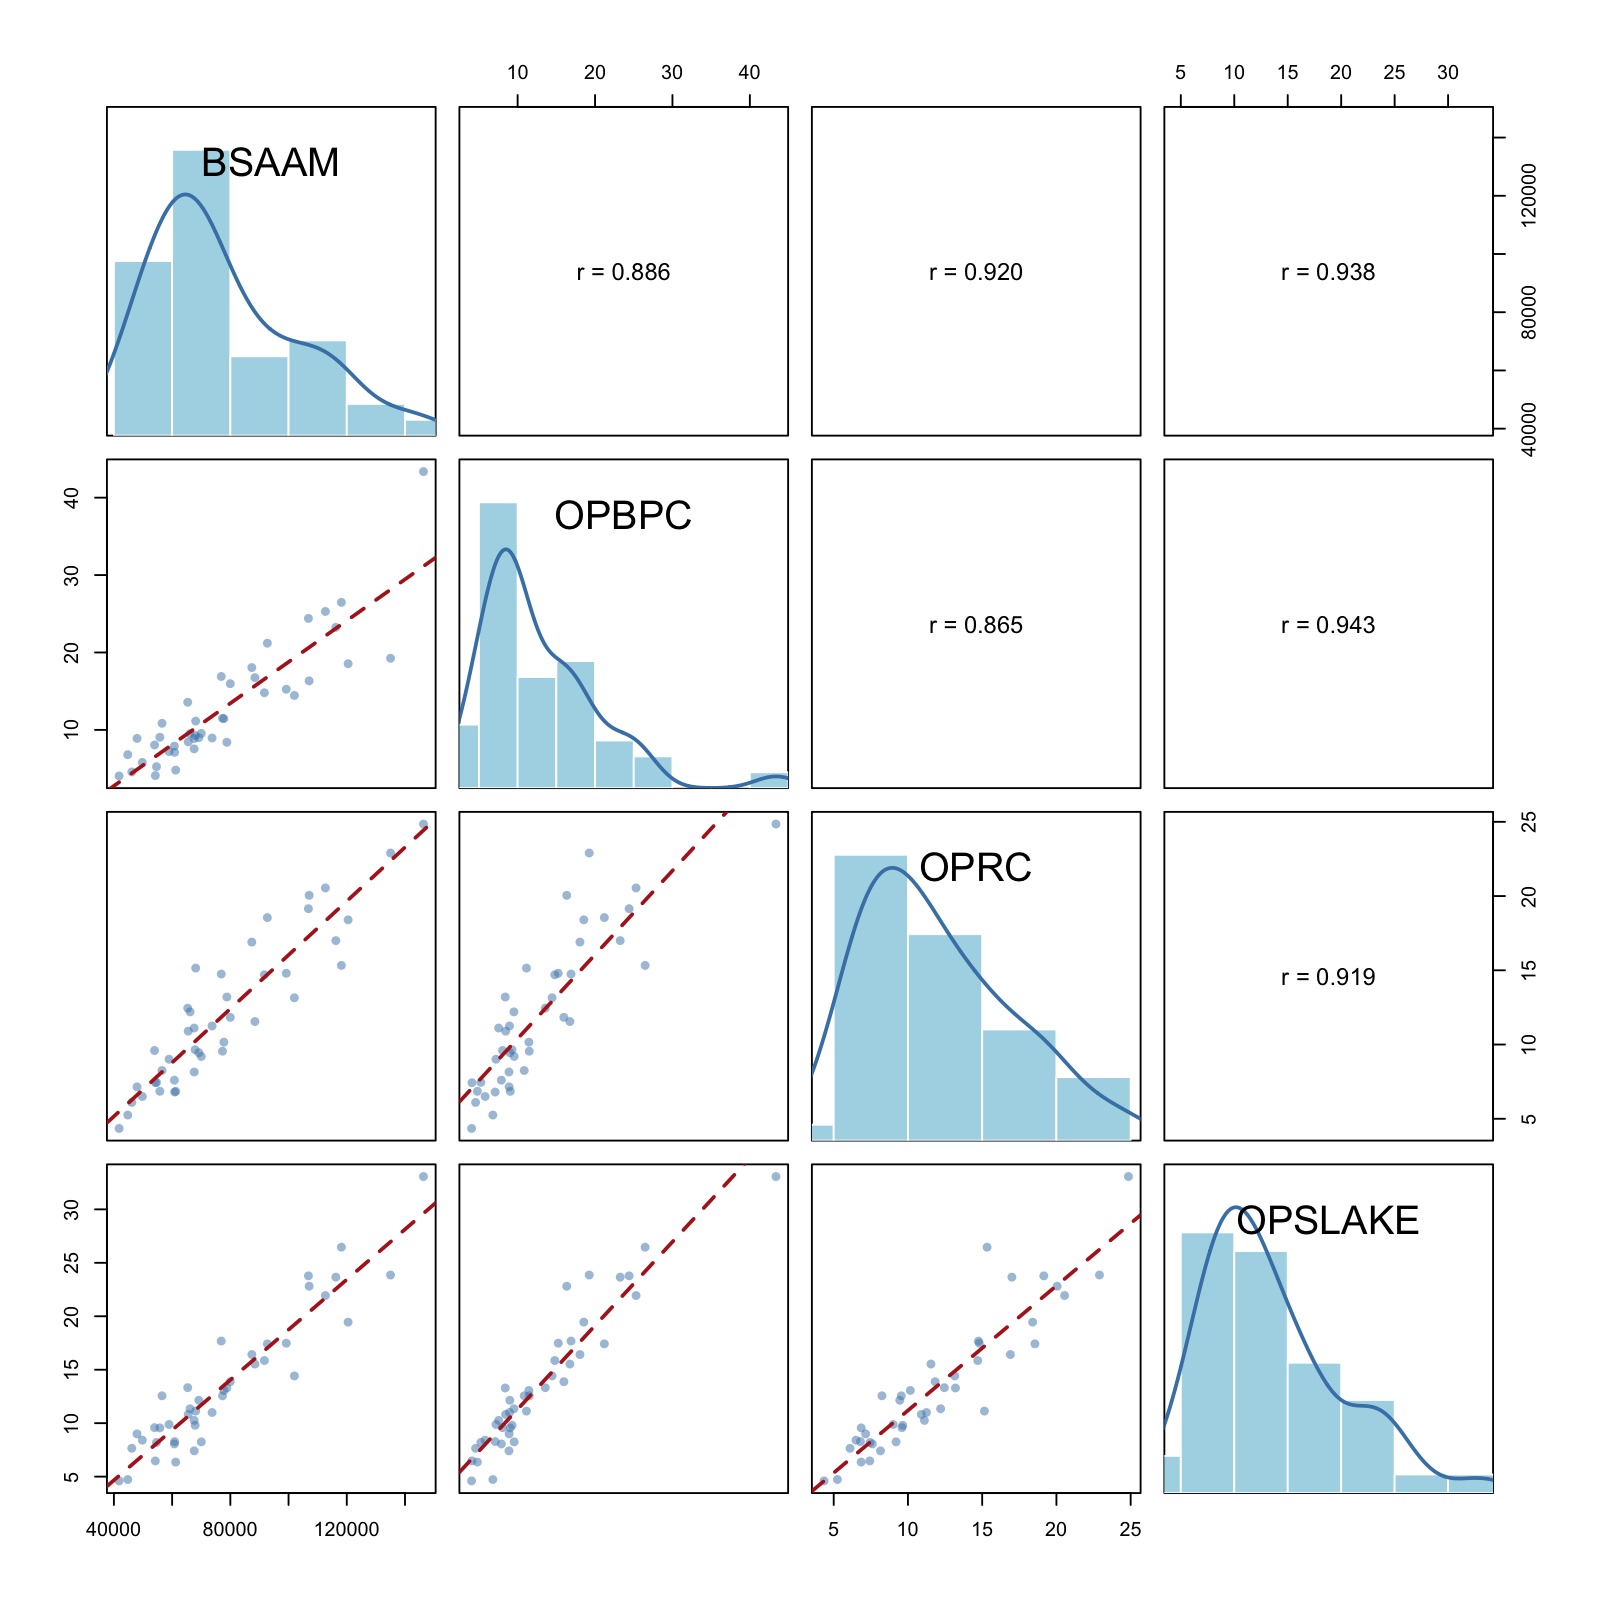
\includegraphics[width=0.65\textwidth]{assets/r-results/problem8-scatter-matrix.png}
\\{\small\color{textgray} 图：\texttt{BSAAM} 与 \texttt{OPBPC}、\texttt{OPRC}、\texttt{OPSLAKE} 的散点图矩阵}
\end{center}

观察散点图矩阵：所有变量两两之间的散点都紧密围绕一条向右上方倾斜的直线，因此相关矩阵中所有相关系数都应当较大且都为正，没有负相关；其中 \texttt{BSAAM} 与 \texttt{OPSLAKE} 的散点最贴近拟合线（相关性最强），与 \texttt{OPRC} 次之，与 \texttt{OPBPC} 相对最松散；回归变量之间也都大且为正，\texttt{OPBPC} 与 \texttt{OPSLAKE} 之间看起来最高。

计算相关矩阵可知：

\begin{center}
\begin{tabular}{lcccc}
\toprule
 & \texttt{BSAAM} & \texttt{OPBPC} & \texttt{OPRC} & \texttt{OPSLAKE} \\
\midrule
\texttt{BSAAM}   & 1.000 & 0.886 & 0.920 & 0.938 \\
\texttt{OPBPC}   & 0.886 & 1.000 & 0.865 & 0.943 \\
\texttt{OPRC}    & 0.920 & 0.865 & 1.000 & 0.919 \\
\texttt{OPSLAKE} & 0.938 & 0.943 & 0.919 & 1.000 \\
\bottomrule
\end{tabular}
\end{center}

于是我们知道，全部相关系数均为大且为正（最小 $0.865$，最大 $0.943$），没有大且为负的相关，且 \texttt{BSAAM} 与 \texttt{OPSLAKE} 的相关（$0.938$）强于 \texttt{OPRC}（$0.920$）和 \texttt{OPBPC}（$0.886$）。
\end{answerbox}

\subsection{}

给出 \texttt{BSAAM} 关于这三个回归变量回归的回归摘要。解释输出中“$t$-values”一列的含义。

\begin{answerbox}
\textbf{解：}

对 \texttt{BSAAM} 关于三个回归变量作多元线性回归（$n=43$），回归摘要如下（R 输出：残差标准误为 $8304$，残差自由度为 $39$；$R^2=0.9017$，调整 $R^2=0.8941$，$F=119.2$，自由度为 $(3,39)$，$p<2.2\times10^{-16}$）：

\textbf{R 代码：}
\begin{lstlisting}[style=rcode]
fit8 <- lm(BSAAM ~ OPBPC + OPRC + OPSLAKE, data = water)
print(summary(fit8))
print(confint(fit8))
t_table <- function(model) {
  tab <- coef(summary(model))
  t_value <- tab[, "Estimate"] / tab[, "Std. Error"]
  data.frame(estimate = tab[, "Estimate"],
             SE = tab[, "Std. Error"], t_value = t_value,
             p_value = 2 * pt(-abs(t_value),
                              df = df.residual(model)))
}
print(t_table(fit8))
print(df.residual(fit8))
\end{lstlisting}

\begin{center}
\small
\begin{tabular}{lrrrrr}
\toprule
 & 系数估计 & 标准误 & $t$-值 & $p$-值 & 95\% 置信区间 \\
\midrule
截距            & 22991.85 & 3545.32 & 6.485 & $<0.001$ & $(15820.78,\ 30162.93)$ \\
\texttt{OPBPC}  & 40.61    & 502.40  & 0.081 & 0.936    & $(-975.59,\ 1056.81)$ \\
\texttt{OPRC}   & 1867.46  & 647.04  & 2.886 & 0.006    & $(558.70,\ 3176.22)$ \\
\texttt{OPSLAKE}& 2353.96  & 771.71  & 3.050 & 0.004    & $(793.03,\ 3914.88)$ \\
\bottomrule
\end{tabular}
\end{center}

即拟合的回归方程为
$$
\widehat{\texttt{BSAAM}}=22991.85+40.61\,\texttt{OPBPC}+1867.46\,\texttt{OPRC}+2353.96\,\texttt{OPSLAKE}.
$$

\textbf{$t$-值列的含义：对各回归系数作双侧 $t$ 检验。}

令 $\beta_1,\beta_2,\beta_3$ 分别对应 \texttt{OPBPC}、\texttt{OPRC}、\texttt{OPSLAKE}，$\beta_0$ 为截距。以下取每个检验的显著性水平为 $\alpha=0.01$。

对每个 $j=0,1,2,3$，分别检验
$$
H_0:\;\beta_j=0
\qquad\text{vs.}\qquad
H_1:\;\beta_j\neq0.
$$

设矩阵 $X$ 包含截距列，令
$$
s^2=\frac{\sum_{i=1}^{43}\hat e_i^2}{43-3-1},
\qquad
\operatorname{SE}(\hat\beta_j)
=s\sqrt{\left[(X^{\mathsf T}X)^{-1}\right]_{j+1,j+1}}.
$$
于是检验统计量为
$$
T_j=\frac{\hat\beta_j-0}{\operatorname{SE}(\hat\beta_j)}.
$$
若 $H_0$ 成立，则
$$
T_j\sim t(n-p-1)=t(39).
$$
回归摘要中的 \texttt{t value} 即 $T_j$ 的观测值。


双侧检验的拒绝域为
$$
|T_j|>t_{\alpha/2}(39)=t_{0.005}(39)
$$
记 $F_{39}$ 为 $t(39)$ 分布的分布函数。观测到 $t_j$ 后，$p$ 值为
$$
p_j=P\bigl(|T|\ge|t_j|\bigr)
=2\bigl[1-F_{39}(|t_j|)\bigr],\qquad T\sim t(39).
$$

\textbf{截距 $\beta_0$：}
$$
p_0\approx1.0993\times10^{-7}.
$$
由于 $p_0<0.01$，拒绝 $H_0:\beta_0=0$，截距显著非零。

\textbf{\texttt{OPBPC} 的系数 $\beta_1$：}
$$
p_1=2[1-F_{39}(0.0808)]\approx0.93599.
$$
由于 $p_1>0.01$，不拒绝 $H_0:\beta_1=0$。控制另外两个变量后，没有充分证据表明 \texttt{OPBPC} 的系数非零。

\textbf{\texttt{OPRC} 的系数 $\beta_2$：}
$$
p_2=2[1-F_{39}(2.8862)]\approx0.00633.
$$
由于 $p_2<0.01$，拒绝 $H_0:\beta_2=0$。控制其他变量后，\texttt{OPRC} 的系数在 $1\%$ 水平下显著非零。

\textbf{\texttt{OPSLAKE} 的系数 $\beta_3$：}
$$
p_3=2[1-F_{39}(3.0503)]\approx0.00410.
$$
由于 $p_3<0.01$，拒绝 $H_0:\beta_3=0$。控制其他变量后，\texttt{OPSLAKE} 的系数在 $1\%$ 水平下显著非零。

\texttt{OPBPC} 与响应变量的边际相关虽高达 $0.886$，但它与另外两个自变量也高度相关，因此边际相关强并不意味着控制其他变量后系数仍显著。
\end{answerbox}

% ==================================================

\section{Problem 9（30 分）}

\texttt{Boston.csv} 收集了可能影响波士顿房价的因素，其中
\texttt{MEDV} 是自有住房的房价中位数，\texttt{CRIM} 是城镇人均犯罪率等。
假设 $Y$ 表示 \texttt{MEDV}，自变量为其他特征，考虑多元线性回归模型。

\subsection{}

计算回归的结果，计算并解释回归总结中 $t$-值的含义。

\begin{answerbox}
\textbf{解：}

对 \texttt{MEDV} 关于其余 13 个特征作多元线性回归（$n=506$），回归摘要如下（R 输出：残差标准误为 $4.745$，残差自由度为 $492$；$R^2=0.7406$，调整 $R^2=0.7338$，$F=108.1$，自由度为 $(13,492)$，$p<2.2\times10^{-16}$）:

\textbf{R 代码：}沿用第8题定义的 \texttt{t\_table} 函数。
\begin{lstlisting}[style=rcode]
boston <- read.csv("Boston.csv")
fit9_full <- lm(MEDV ~ ., data = boston)
print(summary(fit9_full))
print(t_table(fit9_full))
print(df.residual(fit9_full))
\end{lstlisting}


\begin{center}
\small
\begin{tabular}{lrrrr}
\toprule
 & 系数估计 & 标准误 & $t$-值 & $p$-值 \\
\midrule
截距      & $36.4595$ & $5.103$ & $7.144$  & $<0.001$ \\
\texttt{CRIM}    & $-0.1080$ & $0.033$ & $-3.287$ & $0.001$ \\
\texttt{ZN}      & $0.0464$  & $0.014$ & $3.382$  & $0.001$ \\
\texttt{INDUS}   & $0.0206$  & $0.061$ & $0.334$  & $0.738$ \\
\texttt{CHAS}    & $2.6867$  & $0.862$ & $3.118$  & $0.002$ \\
\texttt{NX}      & $-17.7666$& $3.820$ & $-4.651$ & $<0.001$ \\
\texttt{RM}      & $3.8099$  & $0.418$ & $9.116$  & $<0.001$ \\
\texttt{AGE}     & $0.0007$  & $0.013$ & $0.052$  & $0.958$ \\
\texttt{DIS}     & $-1.4756$ & $0.199$ & $-7.398$ & $<0.001$ \\
\texttt{RAD}     & $0.3060$  & $0.066$ & $4.613$  & $<0.001$ \\
\texttt{TAX}     & $-0.0123$ & $0.004$ & $-3.280$ & $0.001$ \\
\texttt{PTRATIO} & $-0.9527$ & $0.131$ & $-7.283$ & $<0.001$ \\
\texttt{B}       & $0.0093$  & $0.003$ & $3.467$  & $0.001$ \\
\texttt{LSTAT}   & $-0.5248$ & $0.051$ & $-10.347$& $<0.001$ \\
\bottomrule
\end{tabular}
\end{center}

\textbf{$t$-值列的含义：对各回归系数作双侧 $t$ 检验。}

与第8题第(2)小问一致，取每个检验的显著性水平为 $\alpha=0.01$。令 $\beta_0$ 为截距，$\beta_1,\ldots,\beta_{13}$ 依次对应上表中的13个自变量。

对每个 $j=0,1,\ldots,13$，分别检验
$$
H_0:\;\beta_j=0\qquad\text{vs.}\qquad H_1:\;\beta_j\neq0.
$$
对斜率系数而言，原假设表示在控制其他12个自变量后，该变量的线性回归系数为零。

设矩阵 $X$ 包含截距列，令
$$
s^2=\frac{\sum_{i=1}^{506}\hat e_i^2}{506-13-1},
\qquad
\operatorname{SE}(\hat\beta_j)
=s\sqrt{\left[(X^{\mathsf T}X)^{-1}\right]_{j+1,j+1}}.
$$
检验统计量为
$$
T_j=\frac{\hat\beta_j-0}{\operatorname{SE}(\hat\beta_j)}.
$$
在经典正态误差线性模型假设下，若 $H_0$ 成立，则
$$
T_j\sim t(n-p-1)=t(492).
$$
R 回归摘要中的 \texttt{t value} 即该统计量的观测值。

令 $P(T>t_{0.005}(492))=0.005$，则双侧检验的拒绝域为：

$$
|T_j|>t_{\alpha/2}(492)=t_{0.005}(492)\approx2.5859.
$$
记 $F_{492}$ 为 $t(492)$ 分布的分布函数，则观测到 $t_j$ 后，双侧 $p$ 值为
$$
p_j=P\bigl(|T|\ge|t_j|\bigr)
=2\bigl[1-F_{492}(|t_j|)\bigr],\qquad T\sim t(492).
$$

例如，对 \texttt{LSTAT} 的系数，
$$
t_{\texttt{LSTAT}}=\frac{-0.5247584}{0.05071528}\approx-10.3471,
\qquad
p_{\texttt{LSTAT}}=2[1-F_{492}(10.3471)]\approx7.777\times10^{-23}.
$$
由于 $|t_{\texttt{LSTAT}}|>2.5859$ 且 $p_{\texttt{LSTAT}}<0.01$，拒绝原假设，控制其他变量后其系数显著非零。

对 \texttt{AGE} 的系数，
$$
t_{\texttt{AGE}}=\frac{0.0006922246}{0.013209782}\approx0.0524,
\qquad
p_{\texttt{AGE}}=2[1-F_{492}(0.0524)]\approx0.95823.
$$
由于 $|t_{\texttt{AGE}}|<2.5859$ 且 $p_{\texttt{AGE}}>0.01$，无法拒绝原假设。

各系数代入后的结果汇总如下（$p$ 值使用 R 的未舍入统计量计算）：
\begin{center}
\small
\begin{tabular}{lrrl}
\toprule
系数对应项 & $t$ 值 & 双侧 $p$ 值 & $\alpha=0.01$ 时的结论 \\
\midrule
截距 & $7.1441$ & $3.283\times10^{-12}$ & 拒绝 $H_0$ \\
\texttt{CRIM} & $-3.2865$ & $0.001087$ & 拒绝 $H_0$ \\
\texttt{ZN} & $3.3816$ & $0.000778$ & 拒绝 $H_0$ \\
\texttt{INDUS} & $0.3343$ & $0.738288$ & 不拒绝 $H_0$ \\
\texttt{CHAS} & $3.1184$ & $0.001925$ & 拒绝 $H_0$ \\
\texttt{NX} & $-4.6513$ & $4.246\times10^{-6}$ & 拒绝 $H_0$ \\
\texttt{RM} & $9.1161$ & $1.979\times10^{-18}$ & 拒绝 $H_0$ \\
\texttt{AGE} & $0.0524$ & $0.958229$ & 不拒绝 $H_0$ \\
\texttt{DIS} & $-7.3980$ & $6.013\times10^{-13}$ & 拒绝 $H_0$ \\
\texttt{RAD} & $4.6129$ & $5.071\times10^{-6}$ & 拒绝 $H_0$ \\
\texttt{TAX} & $-3.2800$ & $0.001112$ & 拒绝 $H_0$ \\
\texttt{PTRATIO} & $-7.2825$ & $1.309\times10^{-12}$ & 拒绝 $H_0$ \\
\texttt{B} & $3.4668$ & $0.000573$ & 拒绝 $H_0$ \\
\texttt{LSTAT} & $-10.3471$ & $7.777\times10^{-23}$ & 拒绝 $H_0$ \\
\bottomrule
\end{tabular}
\end{center}

因此，在各自 $1\%$ 的显著性水平下，除 \texttt{AGE} 和 \texttt{INDUS} 外，其余系数均显著非零。对这两个变量不拒绝原假设，表示控制其他变量后没有充分证据表明其系数非零。

\end{answerbox}

\subsection{}

选取三个自变量，查看针对这三个自变量以及因变量绘制的散点图矩阵。

\begin{answerbox}

选取与房价关系最显著且彼此之间相关性不太高的三个自变量 \texttt{RM}（每套住房平均房间数）、\texttt{LSTAT}（低社会经济地位人口比例）、\texttt{PTRATIO}（师生比），连同因变量 \texttt{MEDV} 绘制散点图矩阵；

\textbf{R 代码：}沿用第8题定义的绘图函数。
\begin{lstlisting}[style=rcode]
boston_vars <- c("MEDV", "RM", "LSTAT", "PTRATIO")
save_pairs(boston[boston_vars], "problem9-scatter-matrix.png")
print(round(cor(boston[boston_vars]), 3))
\end{lstlisting}

\begin{center}
  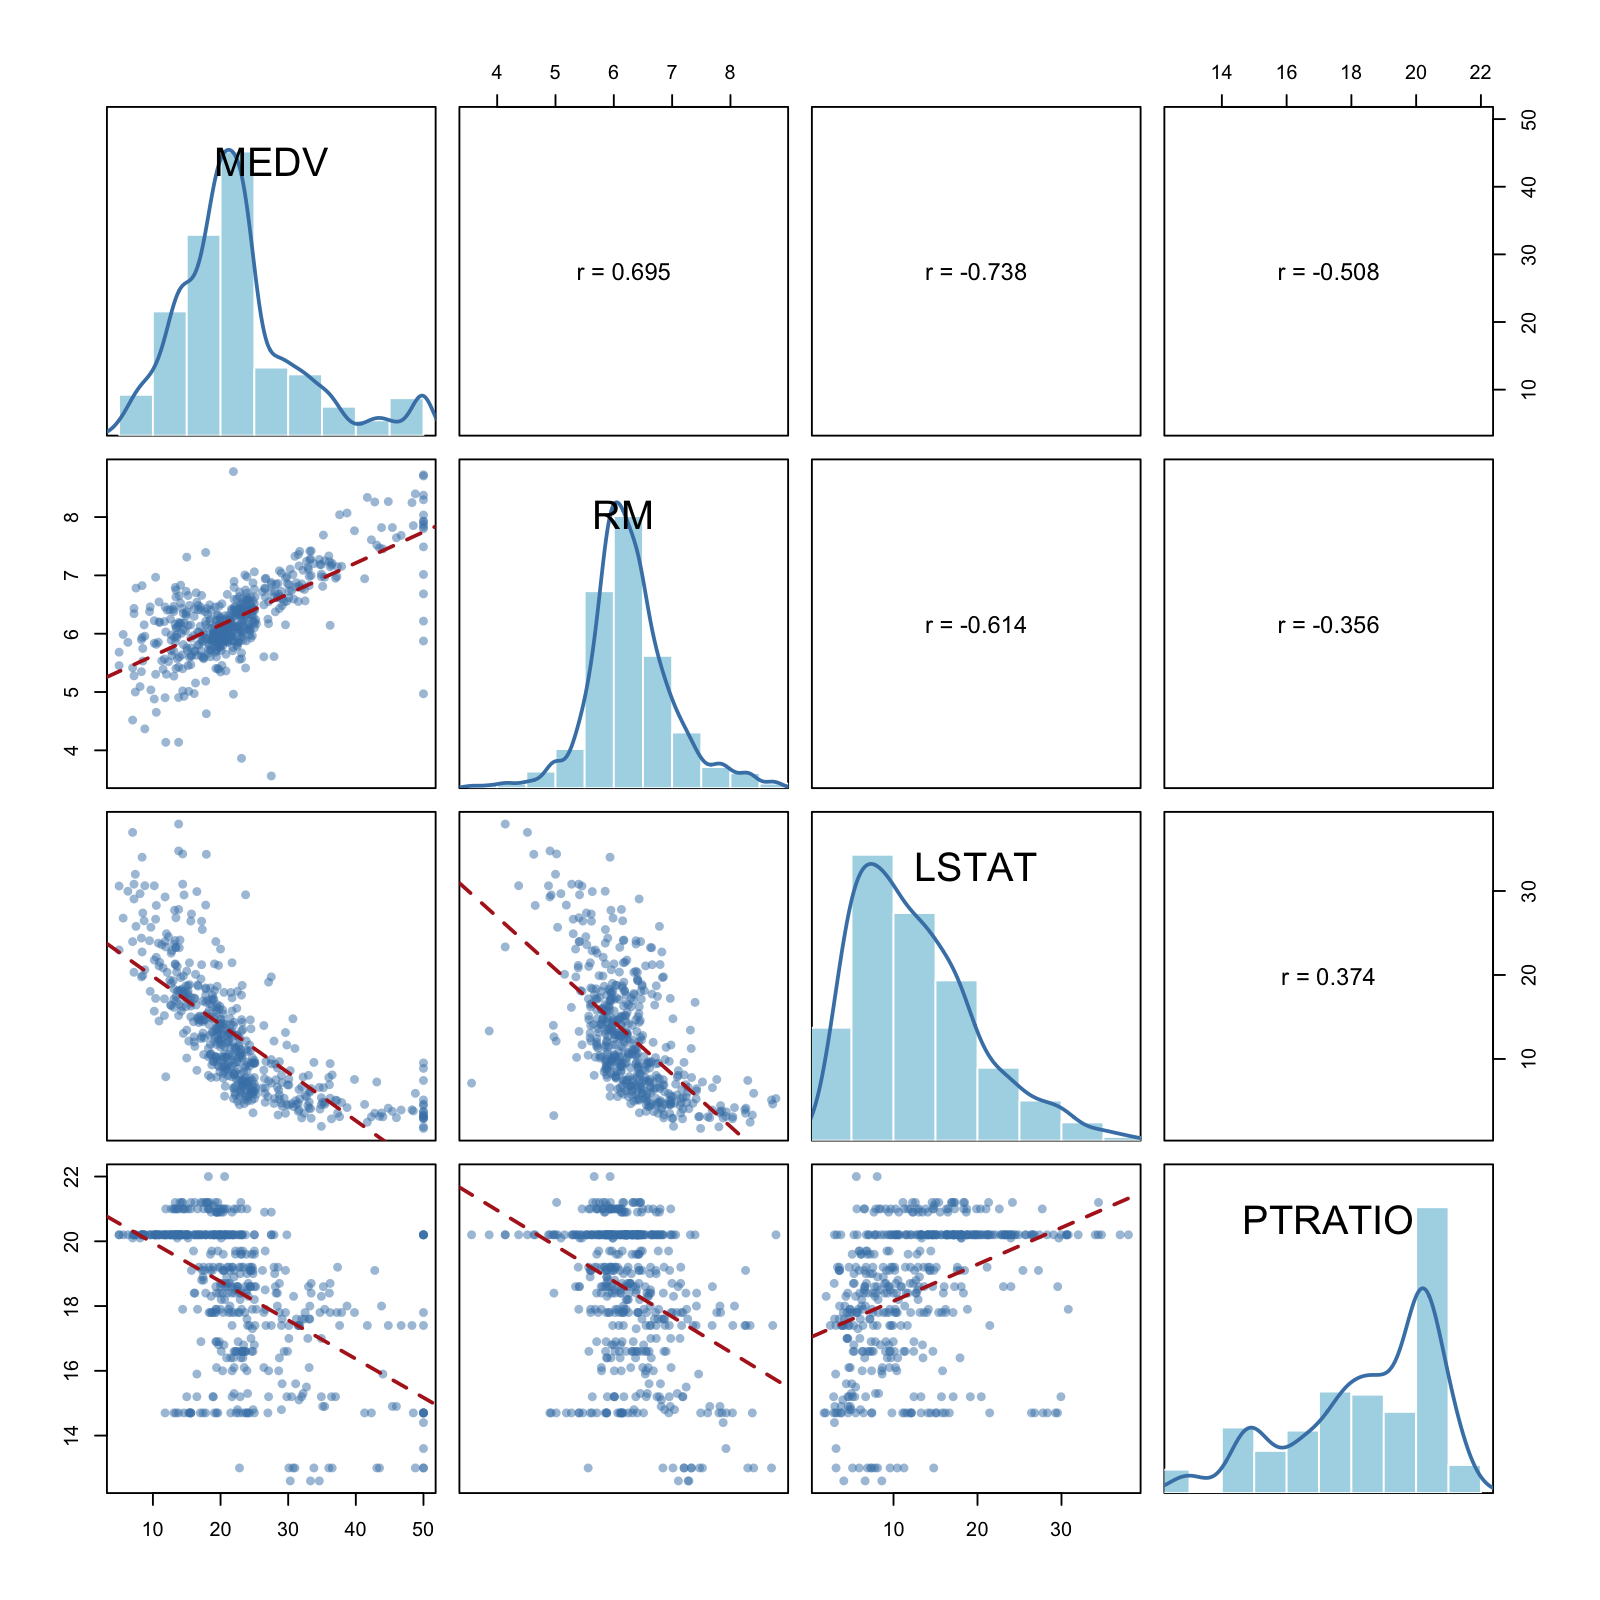
\includegraphics[width=0.86\textwidth]{assets/r-results/problem9-scatter-matrix.png}
\\{\small\color{textgray} 图：\texttt{RM}、\texttt{LSTAT}、\texttt{PTRATIO} 与 \texttt{MEDV} 的散点图矩阵}
\end{center}

R 计算得到 \texttt{MEDV} 与 \texttt{RM}、\texttt{LSTAT}、\texttt{PTRATIO} 的相关系数依次为 $0.695$、$-0.738$、$-0.508$。图中 \texttt{RM} 与房价呈正向关系，\texttt{LSTAT} 与房价呈明显负向关系且存在一定弯曲趋势，\texttt{PTRATIO} 与房价也呈负向关系但散点更分散。三个自变量之间的相关系数分别为 $-0.614$（\texttt{RM} 与 \texttt{LSTAT}）、$-0.356$（\texttt{RM} 与 \texttt{PTRATIO}）、$0.374$（\texttt{LSTAT} 与 \texttt{PTRATIO}）；是否存在多重共线性还需结合下一小问的 VIF 判断。
\end{answerbox}

\subsection{}

分析自变量中有没有多重共线性的情况。如果有，试着去掉某个或某些自变量，
比较回归效果。

\begin{answerbox}

\textbf{(a) VIF }\quad

对全部自变量计算方差膨胀因子，结果如下:

\textbf{R 代码：共线性诊断。}
\begin{lstlisting}[style=rcode]
vif_numeric <- function(model) {
  x <- model.matrix(model)[, -1, drop = FALSE]
  values <- vapply(seq_len(ncol(x)), function(j) {
    auxiliary <- lm(x[, j] ~ x[, -j, drop = FALSE])
    1 / (1 - summary(auxiliary)$r.squared)
  }, numeric(1))
  setNames(values, colnames(x))
}
vif_full <- vif_numeric(fit9_full)
print(sort(vif_full, decreasing = TRUE))
print(cor(boston$RAD, boston$TAX))
\end{lstlisting}

\begin{center}
\small
\begin{tabular}{lc}
\toprule
变量 & VIF \\
\midrule
\texttt{TAX}     & $9.01$ \\
\texttt{RAD}     & $7.48$ \\
\texttt{NX}      & $4.39$ \\
\texttt{INDUS}   & $3.99$ \\
\texttt{DIS}     & $3.96$ \\
\texttt{AGE}     & $3.10$ \\
\texttt{LSTAT}   & $2.94$ \\
\texttt{ZN}      & $2.30$ \\
\texttt{RM}      & $1.93$ \\
\texttt{PTRATIO} & $1.80$ \\
\texttt{CRIM}    & $1.79$ \\
\texttt{B}       & $1.35$ \\
\texttt{CHAS}    & $1.07$ \\
\bottomrule
\end{tabular}
\end{center}

判断标准：VIF $>10$ 通常认为存在较严重的多重共线性。此处 \texttt{TAX} 的 VIF $=9.01$ 已接近阈值，\texttt{RAD} 的 VIF $=7.48$ 也偏高；其余变量 VIF 均 $<5$。进一步查看相关系数可知 \texttt{RAD} 与 \texttt{TAX} 的相关系数高达 $0.910$，是多重共线性的主要来源。

% \textbf{(b) 条件数}\quad
% 用自变量矩阵 $\mathbf{X}$ 的条件数来判断：
% $$
% \kappa=\frac{\sigma_{\max}(\mathbf{X})}{\sigma_{\min}(\mathbf{X})},
% $$
% 其中 $\sigma_{\min}$、$\sigma_{\max}$ 分别为 $\mathbf{X}$ 的最小与最大奇异值。对原始尺度的 13 个自变量计算得
% $$
% \sigma_{\max}=12585.18,\qquad \sigma_{\min}=1.481,\qquad \kappa=8497.94.
% $$
% 按讲义的判据（$\kappa<10$ 无明显共线性，$10\le\kappa\le30$ 中等共线性，$\kappa>30$ 高度共线性），$\kappa=8497.94$ 远大于 $30$，说明自变量存在\textbf{高度多重共线性}。结合 VIF 与 \texttt{RAD}--\texttt{TAX} 的相关系数 $0.910$，可确认二者是共线性的主要来源。

\textbf{(b) 去掉变量后的比较}\quad
鉴于 \texttt{RAD} 与 \texttt{TAX} 高度相关，分别尝试单独去掉 \texttt{RAD}、单独去掉 \texttt{TAX}，以及同时去掉二者后重新拟合。另外，第(1)小问中 \texttt{AGE} 与 \texttt{INDUS} 的 $p$ 值分别为 $0.958$ 和 $0.738$，均大于 $0.01$，因此增加一组从全模型中同时去掉这两个变量、保留 \texttt{RAD} 与 \texttt{TAX} 的对照实验。主要指标对比如下:

\textbf{R 代码：比较全模型与四个简化模型。}
\begin{lstlisting}[style=rcode]
fit9_no_RAD <- update(fit9_full, . ~ . - RAD)
fit9_no_TAX <- update(fit9_full, . ~ . - TAX)
fit9_no_both <- update(fit9_full, . ~ . - RAD - TAX)
fit9_no_AGE_INDUS <- update(fit9_full, . ~ . - AGE - INDUS)
models <- list(full = fit9_full,
               without_RAD = fit9_no_RAD,
               without_TAX = fit9_no_TAX,
               without_both = fit9_no_both,
               without_AGE_INDUS = fit9_no_AGE_INDUS)
model_metrics <- function(model) {
  s <- summary(model)
  v <- vif_numeric(model)
  c(R_squared = s$r.squared,
    adjusted_R_squared = s$adj.r.squared,
    residual_SE = s$sigma, AIC = AIC(model), BIC = BIC(model),
    F_statistic = unname(s$fstatistic["value"]),
    VIF_RAD = unname(v["RAD"]),
    VIF_TAX = unname(v["TAX"]), max_VIF = max(v))
}
print(t(sapply(models, model_metrics)))
print(anova(fit9_no_AGE_INDUS, fit9_full))
\end{lstlisting}

\begin{center}
\small
\setlength{\tabcolsep}{4pt}
\begin{tabular}{lccccc}
\toprule
指标 & 全模型 & 去掉 \texttt{RAD} & 去掉 \texttt{TAX} & \shortstack{去掉 \texttt{RAD}\\与 \texttt{TAX}} & \shortstack{去掉 \texttt{AGE}\\与 \texttt{INDUS}} \\
\midrule
$R^2$         & $0.7406$ & $0.7294$ & $0.7350$ & $0.7293$ & $0.7406$ \\
Adj.\ $R^2$   & $0.7338$ & $0.7228$ & $0.7285$ & $0.7232$ & $0.7348$ \\
残差标准误    & $4.7453$ & $4.8419$ & $4.7920$ & $4.8386$ & $4.7362$ \\
AIC           & $3027.609$ & $3047.033$ & $3036.554$ & $3045.360$ & $3023.726$ \\
BIC           & $3091.007$ & $3106.204$ & $3095.725$ & $3100.305$ & $3078.671$ \\
$F$-statistic & $108.08$ & $110.75$ & $113.93$ & $120.96$ & $128.21$ \\
\texttt{RAD} 的 VIF & $7.48$ & --- & $2.84$ & --- & $6.86$ \\
\texttt{TAX} 的 VIF & $9.01$ & $3.42$ & --- & --- & $7.27$ \\
自变量最大 VIF & $9.01$ & $4.30$ & $4.37$ & $3.95$ & $7.27$ \\
\bottomrule
\end{tabular}
\end{center}

单独去掉 \texttt{RAD} 后，\texttt{TAX} 的 VIF 从 $9.01$ 降至 $3.42$；单独去掉 \texttt{TAX} 后，\texttt{RAD} 的 VIF 从 $7.48$ 降至 $2.84$。两个简化模型中所有自变量的 VIF 均 $<5$，多重共线性问题得到明显缓解。相比之下，单独去掉 \texttt{TAX} 的 Adjusted $R^2$ 更高，残差标准误、AIC 与 BIC 均更低，拟合损失较小。

同时去掉二者后，自变量最大 VIF 进一步降至 $3.95$。相比单独去掉 \texttt{RAD}，其 $R^2$ 略有下降，但 Adjusted $R^2$ 略有上升，AIC 与 BIC 也有所降低，说明在已经去掉 \texttt{RAD} 的情况下，再去掉 \texttt{TAX} 可以用较小的拟合损失换取更简单的模型。不过，该模型的 Adjusted $R^2$、AIC 与 BIC 均不如单独去掉 \texttt{TAX} 的模型。

同时去掉 \texttt{AGE} 与 \texttt{INDUS} 后，$R^2$ 从 $0.740643$ 略降至 $0.740582$（保留四位小数后均为 $0.7406$），Adjusted $R^2$ 从 $0.7338$ 升至 $0.7348$，残差标准误、AIC 与 BIC 均有所降低，说明删除这两个变量几乎没有损失拟合效果，并使模型更简洁。不过，\texttt{RAD} 与 \texttt{TAX} 的 VIF 仍分别为 $6.86$ 和 $7.27$，因此该方案并未充分缓解二者的多重共线性。

为检验同时删除这两个变量是否显著损害拟合，比较该简化模型与全模型，检验 $H_0:\beta_{\texttt{AGE}}=\beta_{\texttt{INDUS}}=0$。部分 $F$ 检验的自由度为 $(2,492)$，统计量为 $0.0573$，$p=0.9443>0.01$，不拒绝 $H_0$，没有充分证据表明这两个变量在控制其余变量后具有联合的额外线性解释能力。这里使用联合检验，而不是仅由两个单独检验均不显著就直接得出联合不显著的结论。

综合来看，若希望通过删除变量缓解多重共线性，前三个简化模型中单独去掉 \texttt{TAX} 更合适；若侧重拟合效果与模型简洁性，同时去掉 \texttt{AGE} 与 \texttt{INDUS} 的模型在本次比较中 Adjusted $R^2$ 最高，AIC 与 BIC 最低，但仍需注意共线性问题。各模型整体 $F$ 检验的自由度不同，不能仅根据 $F$ 值增大判断简化模型更优；样本外预测能力还需交叉验证等方法评估。

% R 的嵌套模型比较 \texttt{anova(fit9\_reduced, fit9\_full)} 给出：简化模型残差自由度为 $493$、RSS 约为 $11558$；完整模型残差自由度为 $492$、RSS 约为 $11079$。两者残差平方和相差 $479.15$，部分 $F$ 检验统计量为 $21.279$，$p=5.071\times10^{-6}$。因此拒绝 $H_0:\beta_{\texttt{RAD}}=0$，删除 \texttt{RAD} 显著损害拟合，不能仅因其 VIF 较高就认定应当删除。两个模型各自的总体 $F$ 值不能直接用来判断哪个模型更好；样本外预测能力还需交叉验证等方法评估。
\end{answerbox}

\end{document}
